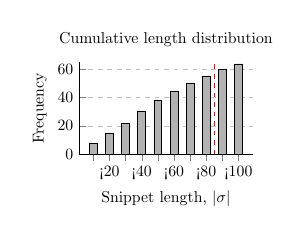
\begin{tikzpicture}[scale=0.57]
  \begin{axis}[
ybar,
bar width=5pt,
xlabel={Snippet length, $|\err\sigma|$},
ylabel={Frequency},
title={Cumulative length distribution},
axis x line*=bottom,
axis y line*=left,
ymin=0,
ymax=65,
xtick=data,
xticklabels={,<20,,<40,,<60,,<80,,<100},
ymajorgrids=true,
grid style=dashed,
width=0.45\textwidth,
height=0.3\textwidth
]

\addplot[fill=black!30] table {
  X Y
  1 7.60
  2 14.52
  3 22.01
  4 30.54
  5 37.82
  6 44.30
  7 49.68
  8 55.21
  9 59.75
  10 63.59
};
\draw[red, dashed] (axis cs:8.5,0) -- (axis cs:8.5,65);
\end{axis}
\end{tikzpicture}
\begin{tikzpicture}[scale=0.57]
\begin{axis}[
ybar,
bar width=5pt,
title={Human repair distance},
xlabel={Edit distance, $\Delta(\err\sigma, \sigma')$},
ylabel={Frequency},
axis x line*=bottom,
axis y line*=left,
xtick=data,
ymajorgrids=true,
grid style=dashed,
xticklabels={,\leq 2,,\leq 4,,\leq 6,,\leq 8,,\leq 10},
ytick={0, 20, 40, 60, 80, 100},
ymin=0,
width=0.45\textwidth,
height=0.3\textwidth
]
\addplot[fill=black!30] table {
X Y
1  31.48
2  47.52
3  54.89
4  60.44
5  63.88
6  66.38
7  68.02
8  70.04
9  71.49
10 72.22
};
\draw[red, dashed] (axis cs:4.5,0) -- (axis cs:4.5,80);
\end{axis}
\end{tikzpicture}
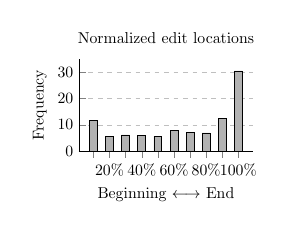
\begin{tikzpicture}[scale=0.57]
\begin{axis}[
ybar,
bar width=5pt,
xlabel={Beginning $\longleftrightarrow$ End},
ylabel={Frequency},
title={Normalized edit locations},
axis x line*=bottom,
axis y line*=left,
ymin=0,
ymax=35,
xtick=data,
xticklabels={,20\%,,40\%,,60\%,,80\%,,100\%},
ymajorgrids=true,
grid style=dashed,
width=0.45\textwidth,
height=0.3\textwidth
]

\addplot[fill=black!30] table {
X Y
10 11.6539
20 5.7252
30 6.2087
40 5.9542
50 5.5980
60 7.9389
70 7.0738
80 6.9466
90 12.4173
100 30.4835
};
\end{axis}
\end{tikzpicture}
%    \begin{tikzpicture}
%      \begin{axis}[
%        ybar,
%        bar width=5pt,
%        title={Intra-patch edit distance},
%        xlabel={Caret distance},
%        ylabel={Frequency},
%        axis x line*=bottom,
%        axis y line*=left,
%        xtick=data,
%        ymajorgrids=true,
%        grid style=dashed,
%        xticklabels={1,2,3,4,5,6,7,8,9,10+},
%        width=0.45\textwidth,
%        height=0.3\textwidth
%      ]
%
%        \addplot table {
%          X Y
%          1 40.66
%          2 15.00
%          3 5.80
%          4 4.86
%          5 4.26
%          6 2.98
%          7 2.05
%          8 2.73
%          9 1.62
%          10 13.64
%        };
%      \end{axis}
%    \end{tikzpicture}
\begin{tikzpicture}[scale=0.57]
\begin{axis}[
legend cell align={left},
legend style={fill opacity=1, draw opacity=1, text opacity=1, draw=lightgray204, legend columns=-1, legend pos=south east},
xlabel={Snippet length, $|\err\sigma|$},
ylabel={Stable region},
title={Stability profile},
ybar,
axis lines*=left,
xtick={0, 10, 20, 30, 40, 50, 60, 70},
ytick={0, 0.2, 0.4, 0.6, 0.8, 1.0},
xticklabels={, {[}10{,}20{)}, , {[}30{,}40{)}, , {[}50{,}60{)}, , {[}70{,}80{)}},
yticklabels={0, 0.2, 0.4, 0.6, 0.8, 1.0},
x tick label style={font=\scriptsize},
ymax=1.0,
ymin=0.0,
bar width=3pt,
grid style=dashed,
ymajorgrids=true,
width=0.45\textwidth,
height=0.3\textwidth
]
\addlegendimage{empty legend}
\addlegendentry{$\Delta(\err\sigma, \sigma')=$}
\addlegendimage{ybar,ybar legend,draw=none,green,fill=green!50}
\addlegendentry{1,}
\addlegendimage{ybar,ybar legend,draw=none,blue,fill=blue!50}
\addlegendentry{2,}
\addlegendimage{ybar,ybar legend,draw=none,orange,fill=orange!50}
\addlegendentry{3}
\addplot[green, fill=green!50] coordinates {(0, 0.80) (10, 0.91) (20, 0.96) (30, 0.97) (40, 0.99) (50, 0.99) (60, 0.99) (70, 0.99)};
\addplot[blue, fill=blue!50] coordinates {(0, 0.35) (10, 0.59) (20, 0.69) (30, 0.73) (40, 0.79) (50, 0.82) (60, 0.84) (70, 0.86)};
\addplot[orange, fill=orange!50] coordinates {(0, 0.23) (10, 0.45) (20, 0.58) (30, 0.66) (40, 0.70) (50, 0.77) (60, 0.78) (70, 0.86)};
\end{axis}
\end{tikzpicture}